% Degrees of freedom needed for the first 1000 eigenvalues: the largest relative
% error over the block against the degrees of freedom, one curve per
% discretisation, with the tolerances as levels and the extrapolations beyond the
% sweep as dotted continuations. Rectangular domain.
%
% The reference is the closed form of the spectrum, so there is no reference
% floor here and none is drawn; on the domains whose reference is a DST run --
% the L-shape, the ellipse minus a quadrant, H and the two drums -- there is one.
%
% This is the one domain carrying a fourth curve. Chebyshev spectral collocation
% builds its operator as a Kronecker sum of one-dimensional differentiation
% matrices, so it needs a domain that fills a tensor-product box and runs here
% and nowhere else in the catalogue.
%
% The two spectral curves fall in quite different ways, and neither is the
% algebraic rate FD and FEM show. The rectangle fills its bounding box, so the
% sine basis the DST operator is built in is its exact eigenbasis, and the only
% thing DST can get wrong is which modes the grid carries: its curve is a real
% error while the grid is one step too coarse for the block -- the thousandth
% eigenvalue is 661, which wants m up to 50 and n up to 25 -- and roundoff
% immediately after, dropping eleven orders of magnitude between two
% neighbouring resolutions. Chebyshev collocation converges instead, and
% exponentially: its error runs from above unity, where the top of the block
% still falls among the spurious high modes, down through 2e-2 to 6e-10 over the
% sweep. Both therefore reach every tolerance asked for within the sweep, and no
% power law is fitted to either -- a straight line through an exponential decay,
% or through a single step, would describe neither.
%
% The DST curve costs nothing to place and the Chebyshev one is dear: the
% collocation matrix is not symmetric, so its eig takes the general QR path, and
% the timing labels on the two curves are the point of the comparison as much as
% their heights are.
%
% Requires in the preamble:
%   \usepackage{graphicx}
%   \usepackage{epstopdf}   % the figure is EPS; needed under pdflatex,
%                           % which then wants -shell-escape. Not needed for
%                           % latex/dvips, which reads EPS directly.
%
% The figure lives next to this file, in results/eigenvalues_dof_requirement/.
% If you \input this snippet from elsewhere, point graphicx at that folder, e.g.
%   \graphicspath{{results/eigenvalues_dof_requirement/}}
% and drop the leading path from the \includegraphics argument below.

\begin{figure}[htbp]
  \centering
  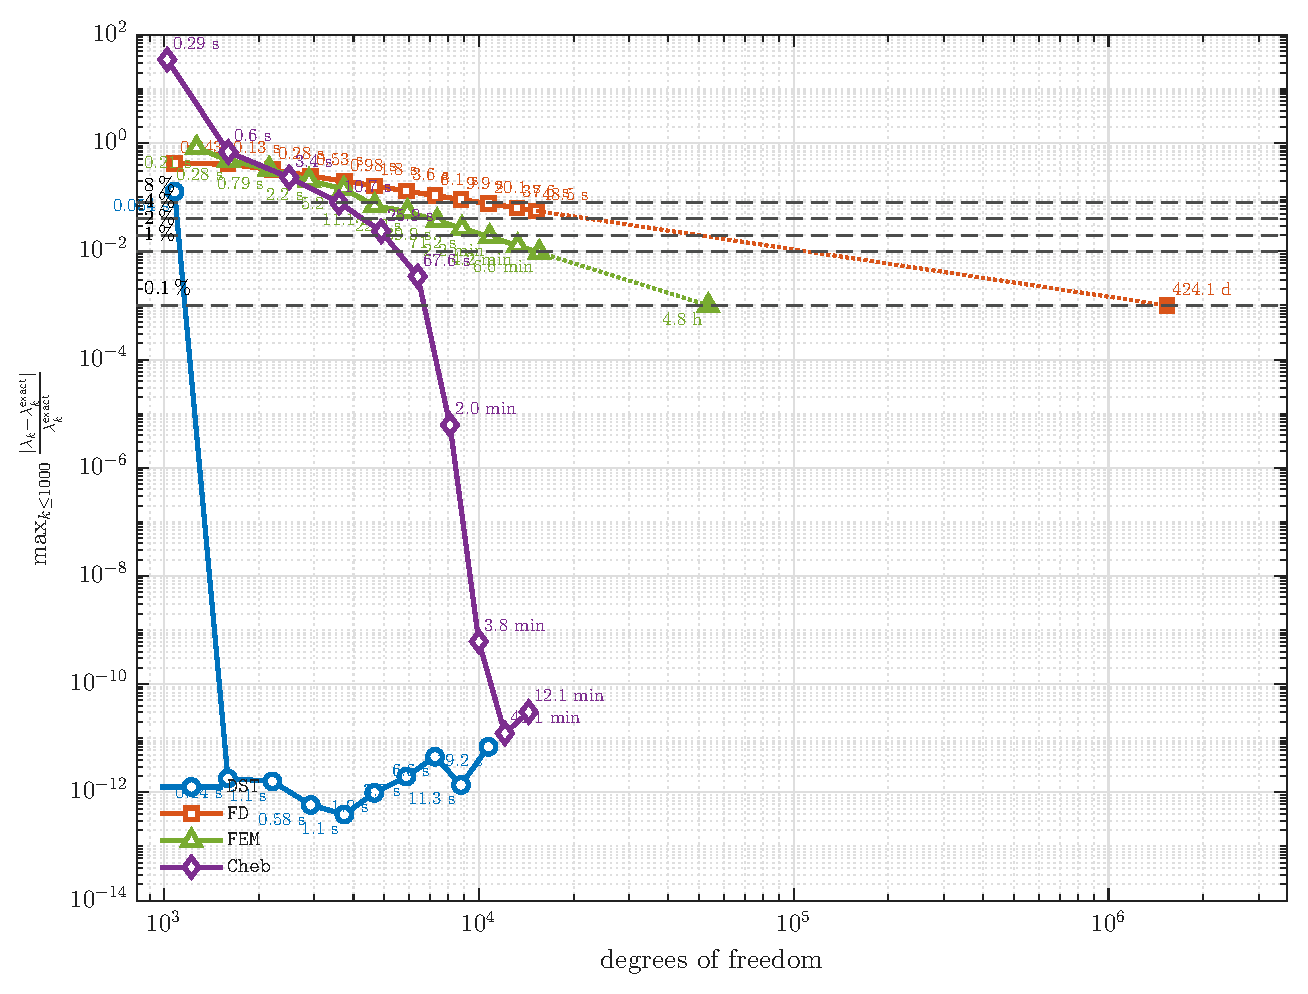
\includegraphics[width=0.85\textwidth]{rectangle_dof_requirement_n1000}
  \caption{Accuracy of the first 1000 eigenvalues of Laplace operator, zero Dirichlet boundary conditions, rectangular domain \texttt{rectangle}. Largest relative error over the whole block of first $1000$ eigenvalues, $\left\{ \lambda_k \right\}_{k=1}^{1000}$, $\max_{k \leq 1000} \frac{|\lambda_k - \lambda_k^{\text{exact}}|}{\lambda_k^{\text{exact}}}$, against the degrees of freedom used by each discretisation of Laplace operator, compared with the exact eigenvalues $\lambda_k^{\text{exact}}$ of the continuous eigenvalue problem. Each marker is labelled with the computation time of the particular run, dotted lines show extrapolated values.}
  \label{fig:dof_requirement_rectangle}
\end{figure}
